\documentclass[tikz]{standalone}
\usepackage{pgfplots}
\usepackage{tikz-3dplot}
\usetikzlibrary{matrix,positioning,arrows,shapes,calc,scopes}
\usetikzlibrary{decorations.markings}
\usetikzlibrary{dsp,chains,fit}
\usetikzlibrary{external}
\usetikzlibrary{graphs}
% colors
\definecolor{snowymint}{HTML}{E3F8D1}
\definecolor{wepeep}{HTML}{FAD2D2}
\definecolor{portafino}{HTML}{F5EE9D}
\definecolor{plum}{HTML}{DCACEF}
\definecolor{sail}{HTML}{A3CEEE}
\definecolor{highland}{HTML}{6D885A}

\tikzstyle{signal}=[arrows={-latex},draw=black,line width=1pt,rounded corners=4pt]

\def\iolen{24pt}
\def\intergape{2pt}

% MLP and CNN
\tikzstyle{netnode}=[circle, inner sep=0pt, text width=22pt, align=center, line width=1.0pt]
\tikzstyle{inputnode}=[netnode, fill=sail,draw=black]
\tikzstyle{hiddennode}=[netnode, fill=snowymint,draw=black]
\tikzstyle{outputnode}=[netnode, fill=plum,draw=black]

% Architecture
\def\layerwidth{90pt}
\def\layerheight{14pt}

\tikzstyle{layer}=[style=block, draw, fill=black!20!white,
    inner sep=1pt,outer sep=0, font=\footnotesize,
    text centered, 
    minimum width=\layerwidth, minimum height=\layerheight]

\tikzstyle{fc}=[style=layer, fill=blue!30!white]
\tikzstyle{conv}=[style=layer, fill=green!30!white]
\tikzstyle{activation}=[style=layer, fill=orange!30!white]
\tikzstyle{pool}=[style=layer, fill=red!30!white]
\tikzstyle{bn}=[style=layer, fill=cyan!30!white]
\tikzstyle{recurrent}=[style=layer, fill=purple!30!white]
\tikzstyle{softmax}=[style=layer, fill=yellow!30!white]
\tikzstyle{point}=[]
\tikzstyle{branch}=[coordinate]

\def\vlayerwidth{30pt}
\def\vlayerheight{3pt}
\def\vblockheight{28pt}

\tikzstyle{vlayer}=[minimum width=\vlayerwidth, minimum height=\vlayerheight]
\tikzstyle{vblock}=[minimum width=\vlayerwidth, minimum height=\vblockheight, text width=1cm, align=center]


\usepackage{mathtools} % Replaced the amsmath package
\usepackage{upgreek}
\usepackage{amssymb}
% \usepackage{mathptmx} % Replaced the times package
% Keep the old calligraphic math font
\DeclareMathAlphabet{\mathcal}{OMS}{cmsy}{m}{n}
\usepackage{amsthm}

\newif\ifcuboidshade
\newif\ifcuboidemphedge
\newif\ifcuboiddrawxdims
\newif\ifcuboiddrawydims
\newif\ifcuboiddrawzdims

\tikzset{
  cuboid/.is family,
  cuboid,
  shiftx/.initial=0,
  shifty/.initial=0,
  dimx/.initial=3,
  dimy/.initial=3,
  dimz/.initial=3,
  scale/.initial=1,
  densityx/.initial=1,
  densityy/.initial=1,
  densityz/.initial=1,
  rotation/.initial=0,
  anglex/.initial=0,
  angley/.initial=90,
  anglez/.initial=225,
  scalex/.initial=1,
  scaley/.initial=1,
  scalez/.initial=0.5,
  front/.style={draw=black,fill=white},
  top/.style={draw=black,fill=white},
  right/.style={draw=black,fill=white},
  shade/.is if=cuboidshade,
  shadecolordark/.initial=black,
  shadecolorlight/.initial=white,
  shadeopacity/.initial=0.15,
  shadesamples/.initial=16,
  emphedge/.is if=cuboidemphedge,
  emphstyle/.style={thick},
  drawzdims/.is if=cuboiddrawzdims,
  dimzval/.initial=C,
  drawxdims/.is if=cuboiddrawxdims,
  dimxval/.initial=W,
  drawydims/.is if=cuboiddrawydims,
  dimyval/.initial=H,
}

\newcommand{\tikzcuboidkey}[1]{\pgfkeysvalueof{/tikz/cuboid/#1}}

% Commands
\newcommand{\tikzcuboid}[1]{
    \tikzset{cuboid,#1} % Process Keys passed to command
  \pgfmathsetlengthmacro{\vectorxx}{\tikzcuboidkey{scalex}*cos(\tikzcuboidkey{anglex})*28.452756}
  \pgfmathsetlengthmacro{\vectorxy}{\tikzcuboidkey{scalex}*sin(\tikzcuboidkey{anglex})*28.452756}
  \pgfmathsetlengthmacro{\vectoryx}{\tikzcuboidkey{scaley}*cos(\tikzcuboidkey{angley})*28.452756}
  \pgfmathsetlengthmacro{\vectoryy}{\tikzcuboidkey{scaley}*sin(\tikzcuboidkey{angley})*28.452756}
  \pgfmathsetlengthmacro{\vectorzx}{\tikzcuboidkey{scalez}*cos(\tikzcuboidkey{anglez})*28.452756}
  \pgfmathsetlengthmacro{\vectorzy}{\tikzcuboidkey{scalez}*sin(\tikzcuboidkey{anglez})*28.452756}
  \begin{scope}[
    xshift=\tikzcuboidkey{shiftx}, 
    yshift=\tikzcuboidkey{shifty}, 
    scale=\tikzcuboidkey{scale}, 
    rotate=\tikzcuboidkey{rotation}, 
    x={(\vectorxx,\vectorxy)}, 
    y={(\vectoryx,\vectoryy)}, 
    z={(\vectorzx,\vectorzy)}]

    \pgfmathsetmacro{\steppingx}{1/\tikzcuboidkey{densityx}}
    \pgfmathsetmacro{\steppingy}{1/\tikzcuboidkey{densityy}}
    \pgfmathsetmacro{\steppingz}{1/\tikzcuboidkey{densityz}}
    \newcommand{\dimx}{\tikzcuboidkey{dimx}}
    \newcommand{\dimy}{\tikzcuboidkey{dimy}}
    \newcommand{\dimz}{\tikzcuboidkey{dimz}}
    \pgfmathsetmacro{\secondx}{2*\steppingx}
    \pgfmathsetmacro{\secondy}{2*\steppingy}
    \pgfmathsetmacro{\secondz}{2*\steppingz}
    \foreach \x in {\steppingx,\secondx,...,\dimx} { 
      \foreach \y in {\steppingy,\secondy,...,\dimy} {   
        \pgfmathsetmacro{\lowx}{(\x-\steppingx)}
        \pgfmathsetmacro{\lowy}{(\y-\steppingy)}
        \filldraw[cuboid/front] (\lowx,\lowy,0.5*\dimz) -- (\lowx,\y,0.5*\dimz) -- (\x,\y,0.5*\dimz) -- (\x,\lowy,0.5*\dimz) -- cycle;
      }
    }
    \foreach \x in {\steppingx,\secondx,...,\dimx} { 
      \foreach \z in {\steppingz,\secondz,...,\dimz} {   
        \pgfmathsetmacro{\lowx}{(\x-\steppingx)}
        \pgfmathsetmacro{\lowz}{(\z-\steppingz-0.5*\dimz)}
        \pgfmathsetmacro{\highz}{(\z-0.5*\dimz)}
        \filldraw[cuboid/top] (\lowx,\dimy,\lowz) -- (\lowx,\dimy,\highz) -- (\x,\dimy,\highz) -- (\x,\dimy,\lowz) -- cycle;
      }
    }
    \foreach \y in {\steppingy,\secondy,...,\dimy} { 
      \foreach \z in {\steppingz,\secondz,...,\dimz} {
        \pgfmathsetmacro{\lowy}{(\y-\steppingy)}
        \pgfmathsetmacro{\lowz}{(\z-\steppingz-0.5*\dimz)}
        \pgfmathsetmacro{\highz}{(\z-0.5*\dimz)}
        \filldraw[cuboid/right] (\dimx,\lowy,\lowz) -- (\dimx,\lowy,\highz) -- (\dimx,\y,\highz) -- (\dimx,\y,\lowz) -- cycle;
      }
    }
    \ifcuboidemphedge
      \draw[cuboid/emphstyle] (0,\dimy,-0.5*\dimz) -- (\dimx,\dimy,-0.5*\dimz) -- (\dimx,\dimy,0.5*\dimz) -- (0,\dimy,0.5*\dimz) -- cycle;%
      \draw[cuboid/emphstyle] (0,\dimy,0.5*\dimz) -- (0,0,0.5*\dimz) -- (\dimx,0,0.5*\dimz) -- (\dimx,\dimy,0.5*\dimz);%
      \draw[cuboid/emphstyle] (\dimx,\dimy,-0.5*\dimz) -- (\dimx,0,-0.5*\dimz) -- (\dimx,0,0.5*\dimz);%
    \fi
    \ifcuboiddrawxdims
      \draw[<->] (0, -0.5, 0.5*\dimz) -- (\dimx, -0.5, 0.5*\dimz) node[below,midway] {$\tikzcuboidkey{dimxval}$};
    \fi
    \ifcuboiddrawydims
      \draw[<->] (-0.5, 0, 0.5*\dimz) -- (-0.5, \dimy, 0.5*\dimz) node[left,midway] {$\tikzcuboidkey{dimyval}$};
    \fi
    \ifcuboiddrawzdims
      \draw[<->] (\dimx, -0.5, -0.5*\dimz) -- (\dimx, -0.5, 0.5*\dimz) node[below right,midway] {$\tikzcuboidkey{dimzval}$};
    \fi

    \ifcuboidshade
      \pgfmathsetmacro{\cstepx}{\dimx/\tikzcuboidkey{shadesamples}}
      \pgfmathsetmacro{\cstepy}{\dimy/\tikzcuboidkey{shadesamples}}
      \pgfmathsetmacro{\cstepz}{\dimz/\tikzcuboidkey{shadesamples}}
      \foreach \s in {1,...,\tikzcuboidkey{shadesamples}} {   
        \pgfmathsetmacro{\lows}{\s-1}
        \pgfmathsetmacro{\cpercent}{(\lows)/(\tikzcuboidkey{shadesamples}-1)*100}
        \fill[opacity=\tikzcuboidkey{shadeopacity},
              color=\tikzcuboidkey{shadecolorlight}!\cpercent!\tikzcuboidkey{shadecolordark}] 
            (0,\s*\cstepy,0.5*\dimz) -- (\s*\cstepx,\s*\cstepy,0.5*\dimz) -- (\s*\cstepx,0,0.5*\dimz) 
              -- (\lows*\cstepx,0,0.5*\dimz) -- (\lows*\cstepx,\lows*\cstepy,0.5*\dimz) -- (0,\lows*\cstepy,0.5*\dimz) -- cycle;
        \fill[opacity=\tikzcuboidkey{shadeopacity},
              color=\tikzcuboidkey{shadecolorlight}!\cpercent!\tikzcuboidkey{shadecolordark}] 
            (0,\dimy,\s*\cstepz-0.5*\dimz) -- (\s*\cstepx,\dimy,\s*\cstepz-0.5*\dimz) -- (\s*\cstepx,\dimy,-0.5*\dimz) 
              -- (\lows*\cstepx,\dimy,-0.5*\dimz) -- (\lows*\cstepx,\dimy,\lows*\cstepz-0.5*\dimz) -- (0,\dimy,\lows*\cstepz-0.5*\dimz) -- cycle;
        \fill[opacity=\tikzcuboidkey{shadeopacity},
              color=\tikzcuboidkey{shadecolorlight}!\cpercent!\tikzcuboidkey{shadecolordark}] 
            (\dimx,0,\s*\cstepz-0.5*\dimz) -- (\dimx,\s*\cstepy,\s*\cstepz-0.5*\dimz) -- (\dimx,\s*\cstepy,-0.5*\dimz) 
              -- (\dimx,\lows*\cstepy,-0.5*\dimz) -- (\dimx,\lows*\cstepy,\lows*\cstepz-0.5*\dimz) -- (\dimx,0,\lows*\cstepz-0.5*\dimz) -- cycle;
      }
    \fi 

  \end{scope}
}


\tdplotsetmaincoords{60}{30}
\newcommand{\bmu}[1]{\mathbf{#1}}           % bold math upright
\newcommand{\xy}{\bmu{u}}

% Define some nicely typesetted words
\newcommand{\CWT}{\ensuremath{{\mathbb{C}}\mathrm{WT}}\xspace} % Nice display of CWT 
\newcommand{\DTCWT}{{\ensuremath{\mathrm{DT}\CWT}}\xspace}
\newcommand{\cifar}{CIFAR-10}
\newcommand{\x}{\times}                     % I don't like having to write out \times so often
\newcommand{\degs}{{\ensuremath{^{\circ}}}\xspace}
\newcommand{\conv}{\ast}
\def\wrt{w.r.t.\xspace}
\def\definedas{\triangleq}
\newcommand{\mycaption}[2]{\caption[#1]{\textbf{#1.} #2}} % Use \macpation{bold font}{rest}

\DeclareMathOperator*{\argmin}{arg\,min}
\DeclareMathOperator*{\argmax}{arg\,max}
% Generic command to make upright words in mathmode 
\newcommand{\F}[1]{\ensuremath{\mathrm{#1}}\xspace}

% And some particularly useful operators
\newcommand{\sgn}{\F{sgn}}
\newcommand{\tr}{\F{trace}}
\newcommand{\diag}{\F{diag}}

% Declare the floor and ceiling operators
\DeclarePairedDelimiter\ceil{\lceil}{\rceil}
\DeclarePairedDelimiter\floor{\lfloor}{\rfloor}

% Define a new command for the euclidean norm of an expression
\newcommand{\norm}[1]{\left\lVert #1 \right\rVert}
\newcommand{\lnorm}[2]{{\left\lVert #1 \right\rVert}_{#2}}
\newcommand{\loss}{L}
\newcommand{\logloss}{\mathcal{L}}
\newcommand{\dydx}[2]{\frac{\partial #1}{\partial #2}}
\newcommand{\conj}[1]{\bar{#1}}
\newcommand{\half}{\frac{1}{2}}
\newcommand{\expected}[2][]{\ensuremath{{\mathbb{E}_{#1}\left[#2\right]}}\xspace}
\newcommand{\drawnfrom}{\ensuremath{\sim}\xspace}
\newcommand{\real}[1]{\F{Re}\left(#1\right)}
\newcommand{\imag}[1]{\F{Im}\left(#1\right)}

% Some vector spaces. These can often be used outside of equations so we will
% add in the ensure math mode. These all have optional arguments which are the
% dimensionality of the space. I.e. if you want to say something belongs to the
% 2 dimensional space of reals, we can call \reals[2]. The Galois spaces need
% to be given the order of their space, so a 3-dimensional binary space would
% be \galois[3]{2}, or simply \binaries[3]
\newcommand{\reals}[1][]{\ensuremath{{\mathbb{R}}^{#1}}\xspace}
\newcommand{\complexes}[1][]{\ensuremath{{\mathbb{C}}^{#1}}\xspace}
\newcommand{\integers}[1][]{\ensuremath{{\mathbb{Z}}^{#1}}\xspace}
\newcommand{\galois}[2][]{\ensuremath{{\mathbb{F}_{#2}}^{#1}}\xspace}
\newcommand{\binaries}[1][]{\galois[#1]{2}\xspace}

\newcommand{\cnnfilt}[4]{h^{(#1)}_{#2}\left(#3, #4 \right)}
\newcommand{\cnnact}[3]{#1\left(#2, #3\right)}
\newcommand{\cnnlact}[4]{#1^{(#2)}\left(#3, #4\right)}

\renewcommand{\vec}[1]{\mathbf{#1}}

% \tikzset{join/.code=\tikzset{after node path={%
% \ifx\tikzchainprevious\pgfutil@empty\else(\tikzchainprevious)%
% edge[every join]#1(\tikzchaincurrent)\fi}}}
% \makeatother
% %
% \tikzset{>=stealth',every on chain/.append style={join},
         % every join/.style={->}}
% \tikzstyle{labeled}=[execute at begin node=$\scriptstyle,
   % execute at end node=$]
\begin{document}

\def \path {dtcwt_scat}
\def \imgpath {dtcwt_scat/images}

% \begin{table}[t]
  \renewcommand{\arraystretch}{1.2}
  \centering
  \mycaption{Hybrid ScatterNet models}{
  Hybrid ScatterNet architectures used for experiments on CIFAR-10 and
  CIFAR-100. For the reference architecture we show the front and back ends. The
  ScatNet A and ScatNet B architectures use the same back end as the reference.
  $N_c$ is the number of output classes; in our experiments we set the channel
  multiplier to be $C=96$.}
  \label{tab:ch5:cifar_arch2}
  \subfloat[Reference 1]{%
    \label{tab:ch5:net_ref}
    \begin{tabular}{l l}
      \toprule
      Layer & Act. Size \\\midrule
      \begin{tabular}{@{}l@{}}
        convA, $w\in \reals[21\x 3 \x 3\x 3]$ \\
        pool1, max pool $2\x 2$ \\
        convB, $w\in \reals[147\x 21\x 3\x 3]$\\ 
        pool2, max pool $2\x 2$ \\
      \end{tabular} &
      \begin{tabular}{@{}l@{}}
        $3\x 32\x 32$ \\ $21 \x 32\x 32$ \\ $21 \x 16\x 16$ \\ $147\x 16\x 16$ \\
        $147\x 8 \x 8$ \\ 
      \end{tabular}\\ \midrule 
      \begin{tabular}{@{}l@{}}
        convC, $w\in \reals[2C\x 147\x 3\x 3]$ \\
        convD, $w\in \reals[2C\x 2C\x 3\x 3]$ \\
        convE, $w\in \reals[4C\x 2C\x 3\x 3]$ \\
        convF, $w\in \reals[4C\x 4C\x 3\x 3]$ \\
        avg pool $8\x 8$ \\
        fc1, $4C\x N_c$
      \end{tabular} & 
      \begin{tabular}{@{}l@{}}
        \\$2C\x 8\x 8$ \\$2C\x 8\x 8$ \\$4C\x 8\x 8$ \\$4C\x 8\x 8$ \\
        $4C$ \\ $N_c$ \\
      \end{tabular}\\
      \bottomrule
    \end{tabular}
    } \\
  \subfloat[ScatNet A Front End]{%
    \label{tab:ch5:net_scatA}
    \begin{tabular}{l l}
      \toprule
      Layer & Act. Size \\\midrule
      \begin{tabular}{@{}l@{}}
        scat1, no $w$ \\
        scat2, no $w$ \\
      \end{tabular} &
      \begin{tabular}{@{}l@{}}
        $3\x 32\x 32$ \\ $21 \x 16\x 16$ \\ $147\x 8 \x 8$ \\
      \end{tabular}\\
      \bottomrule
    \end{tabular}
  }
  \subfloat[ScatNet B Front End]{%
    \label{tab:ch5:net_scatB}
    \begin{tabular}{l l}
      \toprule
      Layer & Act. Size \\\midrule
      \begin{tabular}{@{}l@{}}
        inv1, $A \in \reals[21\x 21]$ \\
        inv2, $A \in \reals[147\x 147]$ \\
      \end{tabular} &
      \begin{tabular}{@{}l@{}}
        $3\x 32\x 32$ \\ $21 \x 16\x 16$ \\ $147\x 8 \x 8$ \\
      \end{tabular}\\
      \bottomrule
    \end{tabular}
  } 
\end{table}
\begin{table}[t]
  \renewcommand{\arraystretch}{1.2}
  \centering
  \mycaption{Hybrid ScatterNet models with convolutional layer
  first}{New front ends for 3 models. The two ScatNet models are the same
  learnable scatternet from \autoref{tab:ch5:net_scatB} but with a small
  convolutional layer (`conv0') before it. ScatNet C ensures the same $147\x 8\x
  8$ output size as the models in \autoref{tab:ch5:cifar_arch2} but ScatNet D
  has a larger output size, allowing for the natural growth of a second-order
  ScatterNet model from $C$ input channels to $49C$ output channels.}
  \subfloat[Reference 2]{%
    \label{tab:ch5:net_ref2}
    \begin{tabular}{l l}
      \toprule
      Layer & Act. Size \\\midrule
      \begin{tabular}{@{}l@{}}
        conv0, $w\in \reals[16\x 3\x 3\x 3]$ \\
        convA, $w\in \reals[50\x 16\x 3\x 3]$ \\
        pool1, max pooling $2\x 2$ \\
        convB, $w\in \reals[147\x 50\x 3\x 3]$\\ 
        pool2, max pooling $2\x 2$ \\
      \end{tabular} &
      \begin{tabular}{@{}l@{}}
        $3\x 32\x 32$ \\ $16\x 32\x 32$ \\ $50 \x 32\x 32$ \\ $50 \x 16\x 16$ \\ $147\x 16\x 16$ \\
        $147\x 8 \x 8$ \\
      \end{tabular}\\
      \bottomrule
    \end{tabular}
  }\\
  \subfloat[ScatNet C]{%
    \label{tab:ch5:net_scatC}
    \begin{tabular}{l l}
      \toprule
      Layer & Act. Size \\\midrule
      \begin{tabular}{@{}l@{}}
        conv0, $w\in \reals[16\x 3\x 3\x 3]$ \\
        inv1, $A \in \reals[50\x 112]$ \\
        inv2, $A \in \reals[147\x 350]$ \\
      \end{tabular} &
      \begin{tabular}{@{}l@{}}
        $3\x 32\x 32$ \\ $16\x 32\x 32$ \\ $50 \x 16\x 16$ \\ $147\x 8 \x 8$ \\
      \end{tabular}\\
      \bottomrule
    \end{tabular}
  }  
  \subfloat[ScatNet D]{%
    \label{tab:ch5:net_scatD}
    \begin{tabular}{l l}
      \toprule
      Layer & Act. Size \\\midrule
      \begin{tabular}{@{}l@{}}
        conv0, $w\in \reals[16\x 3\x 3\x 3]$ \\
        inv1, $A \in \reals[112\x 112]$ \\
        inv2, $A \in \reals[784\x 784]$ \\
      \end{tabular} &
      \begin{tabular}{@{}l@{}}
        $3\x 32\x 32$ \\ $16\x 32\x 32$ \\ $112 \x 16\x 16$ \\ $784\x 8 \x 8$ \\
      \end{tabular}\\
      \bottomrule
    \end{tabular}
  }  
\end{table}

\begin{figure}
  \centering
  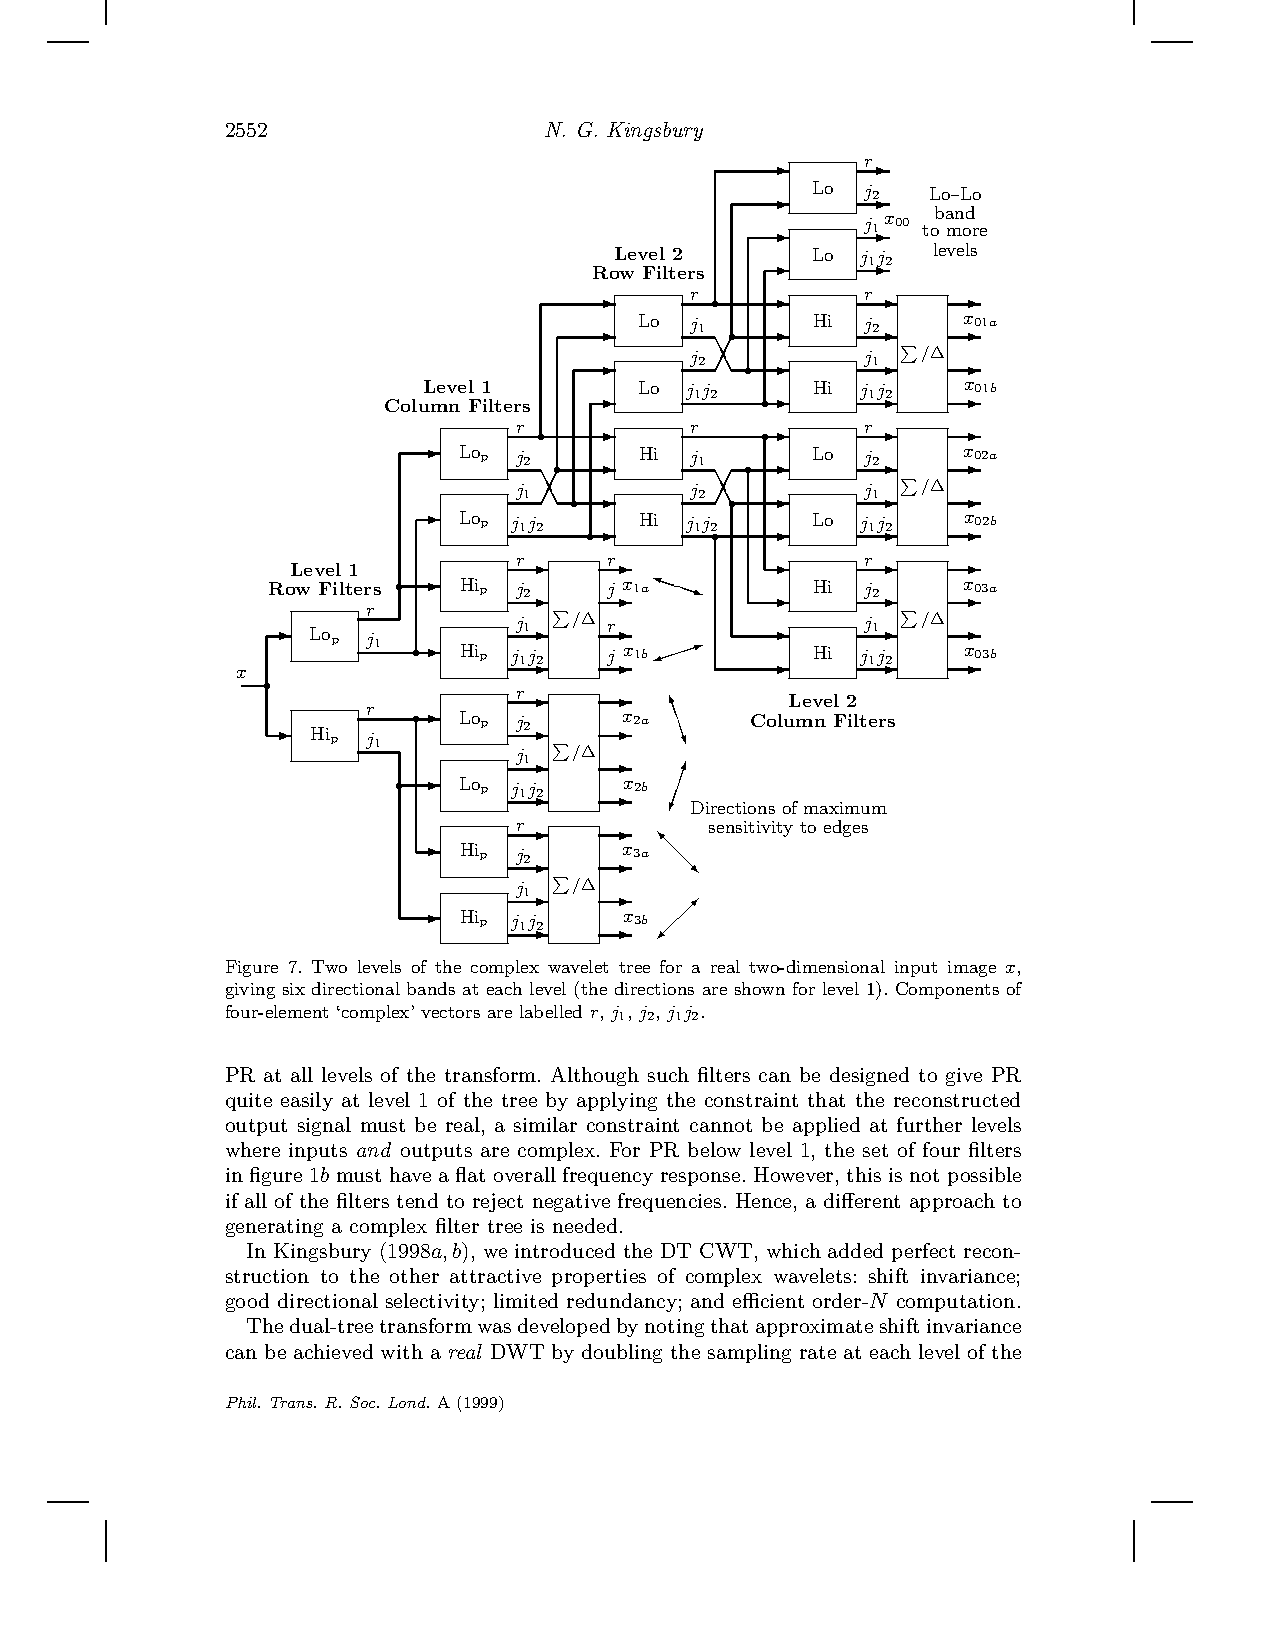
\includegraphics[trim=3cm 11.8cm 4cm 2.5cm, clip]{\imgpath/dtcwt_fb2}
\end{figure}

\end{document}
